\documentclass[a4paper,chapter,kosection,atbegshi,hidelinks,itemph]{oblivoir}
\usepackage[dbl4x6]{fapapersize}
\usepackage{amsmath,amssymb,amsfonts,mdframed,enumitem,graphicx,}
\graphicspath{{./IMG/}}
\setlist{nosep}

\renewcommand\chaptername{강}

\makepagestyle{hf}
\makeevenhead{hf}{\thepage}{}{\itshape\leftmark}
\makeoddhead{hf}{}{}{\thepage}
\makeevenfoot{hf}{}{}{}
\makeoddfoot{hf}{}{}{}
\makepsmarks{hf}{%
\createmark{chapter}{left}{nonumber}{}{}}

\begin{document}
\title{양자정보학 개론\thanks{원문: \url{https://www.scottaaronson.com/qclec.pdf}}}
\author{
    스콧 애론슨\thanks{코리 오스트로브와 파울로 알브스의 큰 도움을 받았다.}, 
    2018년 가을\\
    번역: 김태원
}
\date{\today}
\newpage
\maketitle\thispagestyle{empty}\newpage

\tableofcontents\pagestyle{plain}

\chapter{강의 개요 및 확장 처치-튜링 논제}
\begin{itemize}[label=\(\blacktriangleright\)]
    \item 양자정보학은 천성이 간학문적인 분야다. (물리학, 전산학, 수학, 공학, 철학)
    \item 양자정보학은 단지 유용한 장치나 알고리즘의 발명만이 아니라 양자역학적 작용의 명료화에 관한 것이기도 하다.
    \begin{itemize}
        \item 양자역학으로 할 수 있느냐 없느냐는 물음을 던지기 위한 것이자
        \item 양자역학 자체의 본성에 대한 더 나은 이해를 독려하기 위한 것이다.
    \end{itemize}
    \item 애론슨 교수는 양자정보학 연구의 이론적인 극단에 헌신한다.
    \item 이론가들은 실험가들이 만드는 것을 알리고 이는 다시 이론가들의 질문에 영향을 미친다.
\end{itemize}\hfill\break
오늘은 물리적 세계에 관해 ``자명한" 진술들을 명시한다.
그런 다음 양자역학이 이들 진술 가운데 몇몇만 놔두고 나머지는 뒤엎어 버리는 광경을
목도할 텐데, 이들 진술 간의 차이란 종종 아주 미묘하다!
우선...\hfill\break

\begin{description}[leftmargin=0cm]
    \item[\textbf{확률}\;] 
        $(P\in[0,1])$는 세상의 불확실성을 나타내는 표준적인 방법이다. 
        확률은 아래 같은 일련의 공리를 따라야 한다.
        \begin{itemize}[label=$\blacktriangleright$]
            \item  상호배타적이며 포괄적인 사건{\footnotesize mutually exclusive
            exhaustive events} $n$개의 집합에 대해  
                확률들의 합은 $P_1+P_2+\cdots+P_n=1$을 만족한다.
            \item 임의의 사건에 대한 확률은 $P_i\geq0$을 만족한다.
        \end{itemize}
        \begin{align*}\pmb{\vdots}\end{align*}
\end{description}

\pagestyle{hf}
두 점이 하나의 슬릿을 지닌 장벽으로 구분되어 있다고 하자.
우리는 입자가 한 점에서 다른 점으로 이동하는 확률을 측정하고자 한다.
경로를 늘리면 (다시 말해 또 다른 슬릿을 개방하면) 다른 쪽에 도달할 가능성이 증가,
아니 적어도 감소하지는 않을 것은 분명하다.
확률이 \textbf{단조}{\footnotesize monotone}라고 말하여 이런 성질을 가리킬 수 있다.
    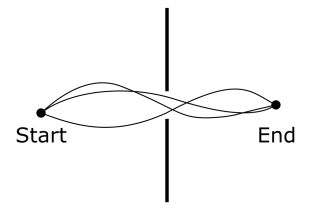
\includegraphics[width=0.25\textwidth]{iqis1_001}
\end{document}
